本文は内側半径1mの円と外側半径2mの円で作られた幅1mの円形コースで実験する.
内側のコース壁を薄青色に塗って,
外側のコース壁を青色の縞模様としている.
時計回りロボット4台と反時計回りロボット4台を2つずつセットにしてコースの中にランダムに置いて,
約8分間実験した.ロボットが自分の向きを判断できるため,


ロボットが破線1から反時計回りで破線2まで移動して,$\theta$が0から$\pi$に変わる.
破線1から時計回りで破線2まで移動して,$\theta$が0から$-\pi$に変わる.
$R$はロボットからコース中心までの距離である(Fig.\ref{courseshitar}).
それに,ロボットが反時計回りで破線1を通過したら,通過回数$n_{ij}$が+1,
ロボットが時計回りで破線1を通過したら,通過回数$n_{ij}$が-1になる.
次,ロボット一台ずつ,各自の$n_{ij}$を計測して,
各ロボットの通過回数の絶対値を足し算して,1回の実験の通過回数になる.
$T_i$は$i$番目の実験の1方向走行流になる時間です(先行研究\cite{li}の$T_{\rm 1d}$と同じ,単位:min),
$n_{ij}$が$T_i$以内の通過回数です,1方向走行流になた後の通過回数を捨てた.
(\ref{eq:flow})式で$i$番目の実験の流量$Q_i$を求めて,
(\ref{eq:flow_ave})式で流量の平均値を求める.
本研究の流量が対面流の流量である.
$j$はロボットの番号で,
$k$はロボットの台数です(今回の実験で1から8まで合計8台ロボットを使ったので,$k=8$.

$w$がコースの幅(単位:m),
$N_{\rm exp}$は全実験回数を表す.

ロボットが渋滞状態を解消する能力も比較するため,2つロボットをペアとして,
ランダムの初期配置(Fig.\ref{randstart})と渋滞の初期配置(Fig.\ref{crowdstart})の実験を行った

\vspace{-1mm}
\begin{figure}[h]
        \centering
        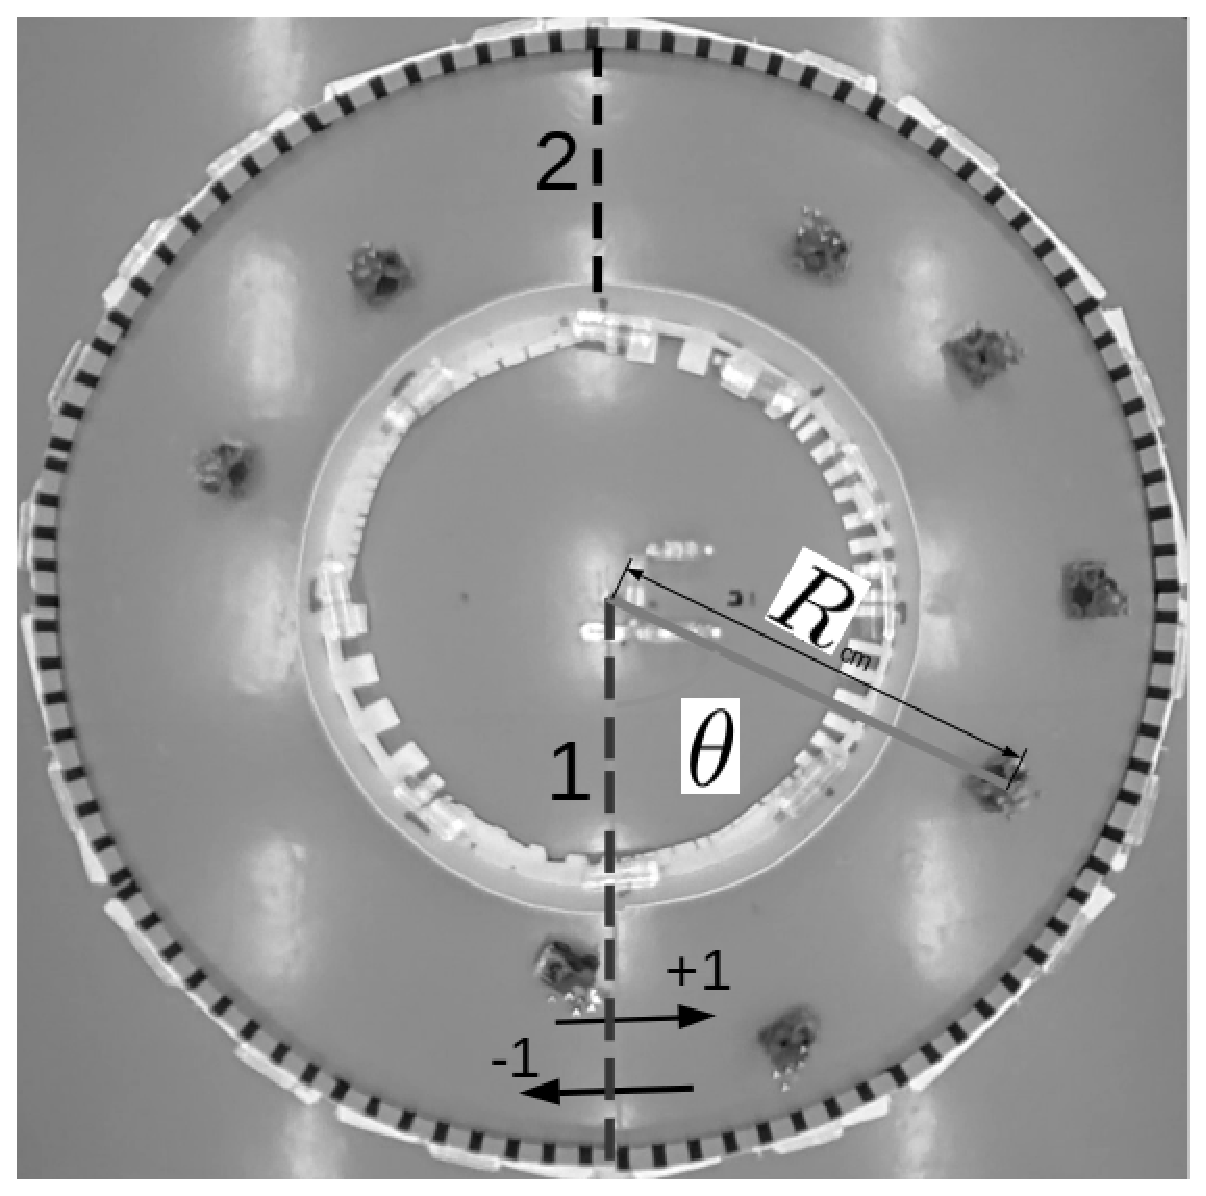
\includegraphics[width=0.6\linewidth]{shitaR.eps}
        \caption{実験の様子(俯瞰図)と$\theta$の説明}
        \label{courseshitar}
\end{figure}

\vspace{-2mm}
\begin{eqnarray}
Q_i &=& \frac{\sum_{j=1}^{k} |n_{ij}|}{wT_i}
\label{eq:flow} \\
\bar{Q} &=& \frac{1}{N_{\rm exp}}\sum_{i=1}^{N_{\rm exp}} Q_i
\label{eq:flow_ave} 
\end{eqnarray}

\vspace{-1mm}
\begin{figure}[h]
    \begin{minipage}{0.49\linewidth}
        \centering
        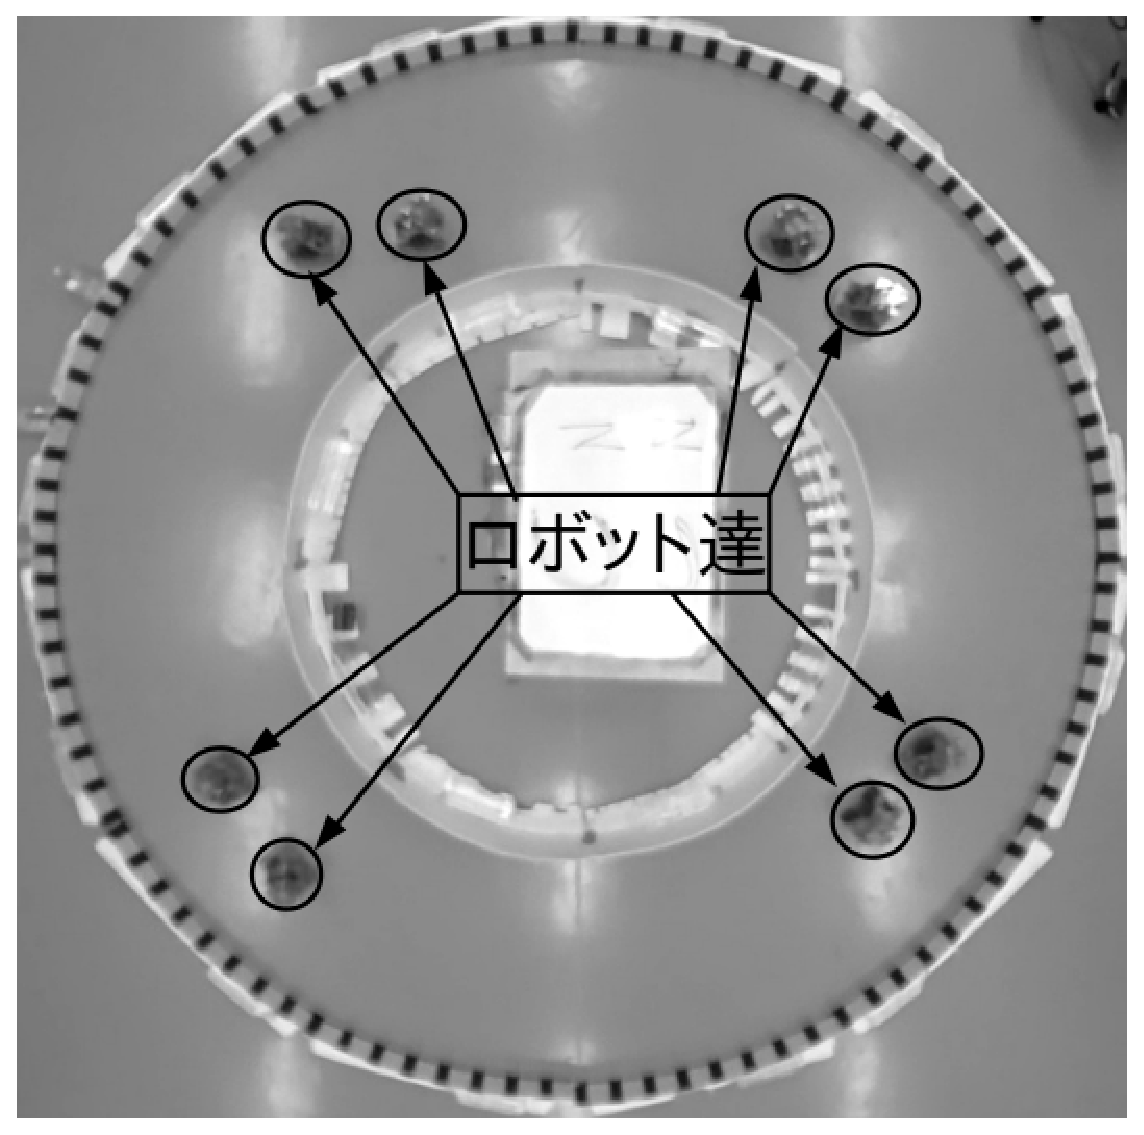
\includegraphics[width=1.0\linewidth]{startrand.eps}
        \caption{ランダムの初期配置}
        \label{randstart}
    \end{minipage}
    \begin{minipage}{0.49\linewidth}
        \centering
        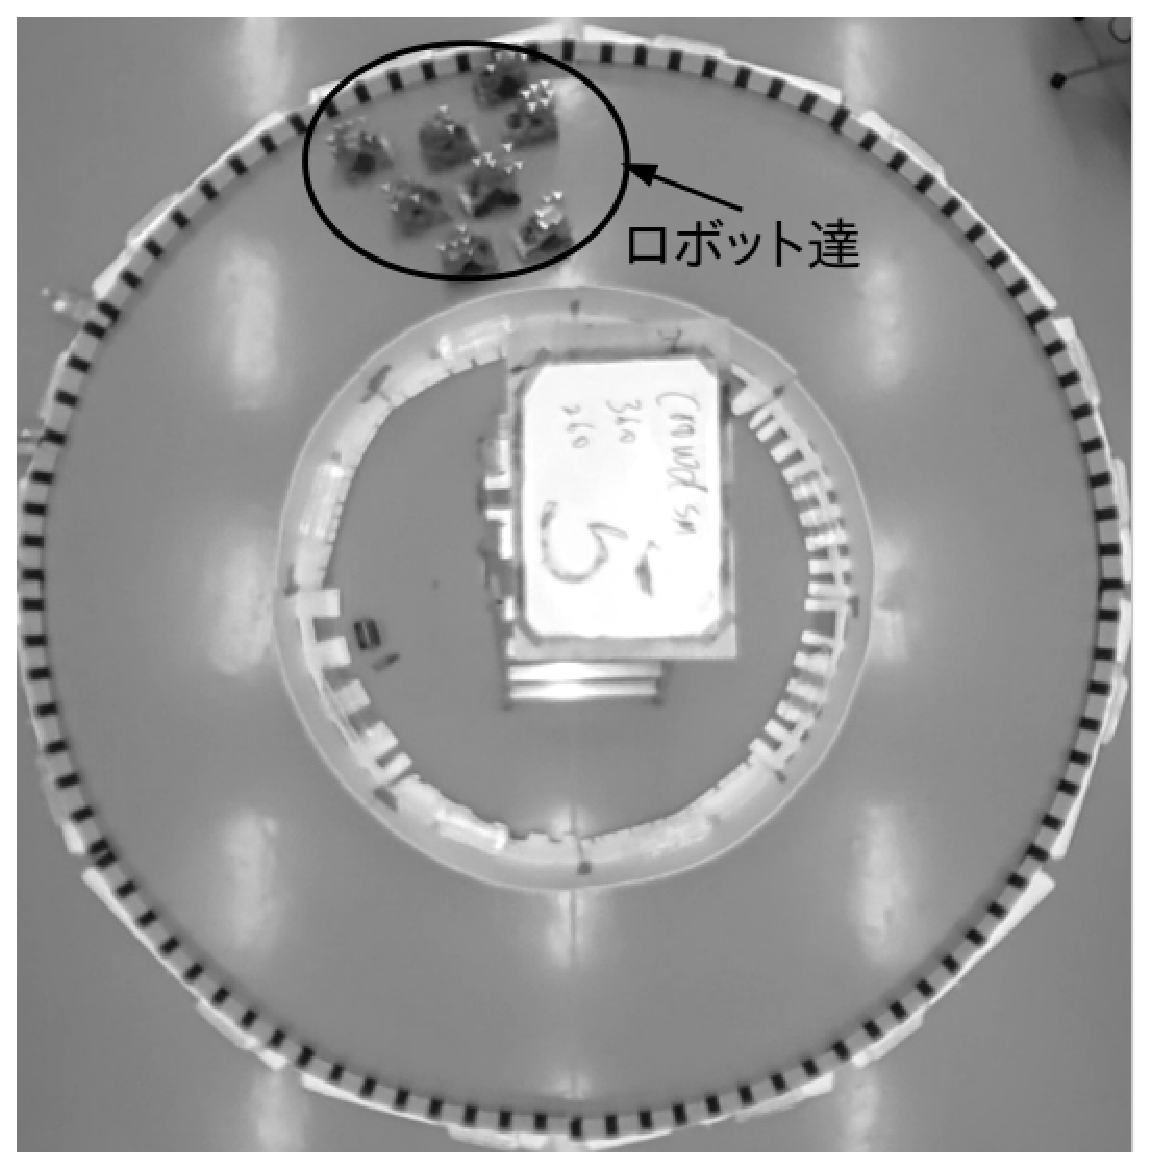
\includegraphics[width=1.0\linewidth]{start_crowd.eps}
        \caption{渋滞の初期配置}
        \label{crowdstart}
    \end{minipage}
\end{figure}
